\documentclass[
  journal=largetwo,
  manuscript=Practica-Dos,
  year=2024-1, % No olivdar cambiar la fecga
  volume=37,
  spanish, % Agrega la opción para el idioma español
]{cup-journal}

\usepackage[english, spanish]{babel}
\usepackage{blindtext}
\usepackage{amsmath}
\usepackage[nopatch]{microtype}
\usepackage{booktabs}
\usepackage{listings}
\usepackage{hyperref} 
\usepackage{matlab-prettifier}

\title{Resolución Espacial y de Intensidad}

\author{Ortiz Castañeda José Ramón}
\affiliation{Facultad de Ciencias, UNAM}
\email{ramon.o@ciencias.unam.mx}


\addbibresource{example.bib}
\keywords{keyword entry 1, keyword entry 2, keyword entry 3} %% First letter not capped

\begin{document}

\begin{abstract}
La resolución espacial y de intensidad son propiedades fundamentales a considerar en el procesamiento digital de imágenes. La resolución espacial se refiere a la cantidad total de píxeles que definen la nitidez con que se pueden representar los detalles en una imagen. Mientras que la resolución de intensidad se refiere a la cantidad de niveles de gris que puede almacenar cada píxel, lo cual afecta el rango dinámico y contraste de la imagen.
\end{abstract}

\noindent \textbf{Objetivos}
\begin{itemize}
    \item Observar de manera experimental los efectos de la manipulación de la resolución y cuantización de una imagen.
    \item Familiarizarse con la manipulación de las imágenes.
    \item Comprender la noción de adyacencia de píxeles y distancia entre píxeles de una imagen.
\end{itemize}

\section{Introducción}
La resolución espacial se define como la capacidad de una imagen para representar el detalle más pequeño discernible. Esta medida puede expresarse de diversas formas, siendo comunes las unidades de líneas por distancia y los píxeles por unidad de medida. Una definición ampliamente utilizada de resolución de imagen es el número máximo de pares de líneas discernibles por unidad de distancia. Por otra parte, la resolución de intensidad hace referencia al cambio más pequeño discernible en el nivel de intensidad o niveles de gris. Desde una perspectiva de hardware, el número de niveles de intensidad suele ser una potencia de dos. El valor más utilizado es de 8 bits, y será la unidad que emplearemos en el desarrollo de esta práctica.

Para llevar a cabo esta práctica, se decidió trabajar con imágenes capturadas a lo largo del último año utilizando un teléfono celular. En el primer ejercicio, se usará una fotografía de la estatua ecuestre de Carlos IV ubicada en el centro histórico de la Ciudad de México. La imagen original [Figure 1] ha sido adaptada a una imagen en escala de grises con una resolución de 1024x1024 píxeles.

\begin{figure}
\centering
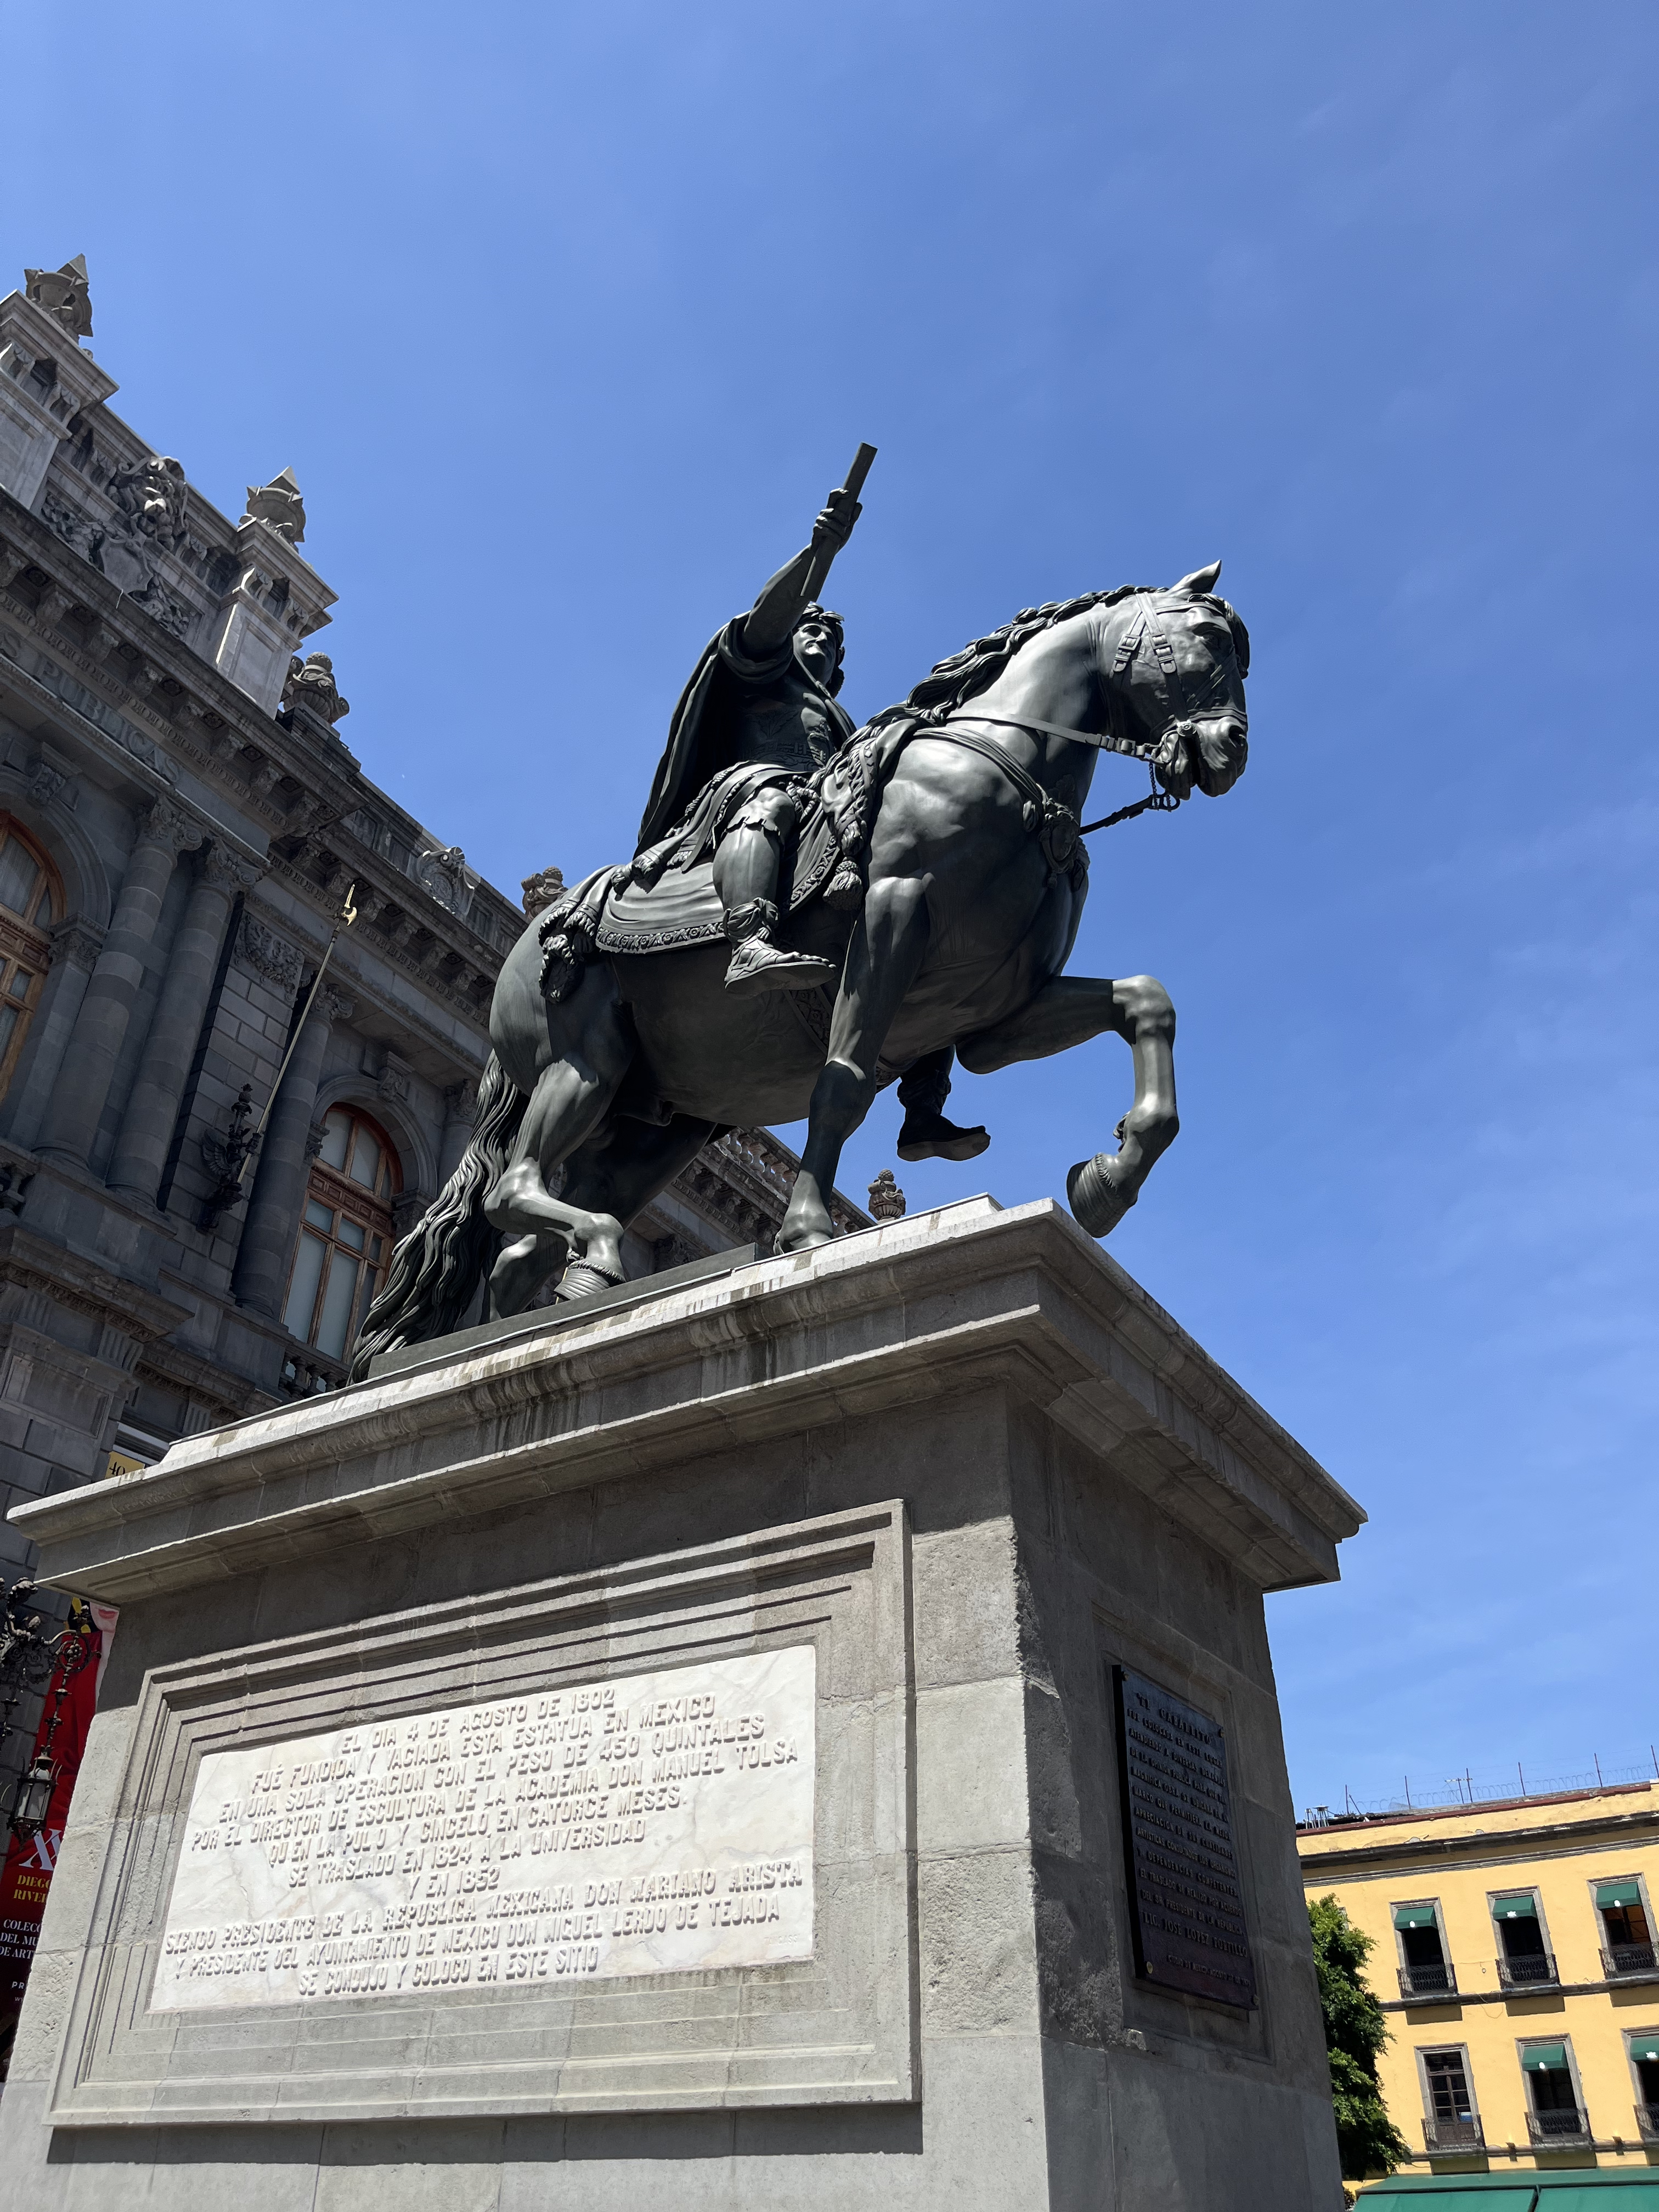
\includegraphics[width=0.4\linewidth]{Practica02/Imagenes/EX01-01.jpg}
\caption{Carlos IV, capturada con gran angular a una resolución de 3024 x 4032 píxeles. El espacio de color es RGB.}
\label{fig_sim}
\end{figure}


\section{Desarrollo}


\subsection{Ejercicio Uno}

Busca una imagen de 1024x1024 pixeles en 256 niveles de gris. Reduce su resolución espacial a 512x512, 256x256, 128x128 y 64x64 pixeles. 

Cuando se reduce la resolución espacial de una imagen, se disminuye el número de píxeles, lo que resulta en una imagen más pequeña en términos de dimensiones físicas y en una pérdida de detalles finos. Esto puede ser útil cuando se necesita reducir el espacio de almacenamiento de una imagen o cuando se quiere acelerar el procesamiento de la imagen ya que hay menos datos para procesar. Para la resolución de este inciso se define una función que recibe como parámetros dos atributos: 

\begin{itemize}
    \item Una matriz de 1024 x 1024 elementos que varían en un rango de 0 a 255, representando la intensidad o escala de grises correspondiente a la información de la imagen original.
    \item Un entero $n$ con las nuevas dimensiones a la que se escalará la Imagen. Los valores que se esperan recibir son: 512, 256, 128 y 64.
\end{itemize}

Cuando se hace una llamada a la función, lo primero que hace es crear una variable auxiliar que contiene el resultado de la división de la longitud de la imagen original (1024) sobre la nueva dimensión $n$. Simultáneamente, inicializamos una matriz de tamaño $n\:\times \:n$.

Se inicia un bucle for anidado, donde el bucle externo itera a través de las filas de la matriz de la nueva imagen y el bucle  interno itera a través de las columnas. Dentro de los bucles se realiza una asignación que calcula las coordenadas en la imagen original que se mapearán a la posición (i, j) de la nueva imagen. Finalmente, se devuelve la matriz que representa la imagen escalada.

\subsection{Ejercicio Dos}
Despliega las cuatro imágenes anteriores en tamaño real (replicar la imagen de las notas Tema 2 DE, pag 5).

\begin{figure}[hbt!]
  \centering
  \includegraphics[width=1\linewidth]{Practica02/Imagenes/EX02-FINAL.pdf}
  \caption{(A) Imagen de 1024x1024 píxeles en 256 niveles de gris, (B) imagen de 512x512 píxeles, (C) imagen de 256x256 píxeles, (D) imagen de 128x128 píxeles, (E) imagen de 64x64 píxeles. Para consultar la imagen original \href{https://drive.google.com/file/d/15F7JUApDnW06WUOVy-UCVoGNYzVpQE6U/view?usp=sharing}{haga click aquí}.}
  \label{fig_sim}
\end{figure}





\subsection{Ejercicio tres}
Haz un zoom a 1024x1024 pixeles de las cuatro imágenes obtenidas en el inciso 1 usando el método del vecino más cercano.

Se calcula el ratio dividiendo el tamaño de la nueva imagen 1024 por la longitud de la imagen original. El ratio es utilizado para determinar cómo mapear los píxeles de la imagen original a los píxeles correspondientes en la nueva imagen. Se obtienen las posiciones interpoladas mediante un ciclo for: se hace uso de la función ceil para redondear el resultado de la división entre i y ratio. 

Definimos variables para la nueva imagen y una matriz auxiliar que nos servirán para mapear los píxeles: en el primer bucle se recorren los píxeles de la imagen original. Para cada píxel en la fila i de la imagen original, se obtiene el índice correspondiente de la posición interpolada en la columna j de newImage. Se asigna el valor del píxel original a dicha posición en newImage. En el segundo bucle se recorren todas las posiciones en auxiliarMatrix. Para cada posición en la fila i y la columna j, se obtiene el índice correspondiente de la posición interpolada en la fila i de newImage. Se asigna el valor de newImage a dicha posición en auxiliarMatrix. Por ultimo se le asigna a newImage la matriz auxiliarMatrix. En la figura tres se pueden ver las imágenes  obtenidas en el inciso uno.

\begin{figure}
\centering
\includegraphics[width=1\linewidth]{Practica02/Imagenes/EX03.pdf}
\caption{(A) Imagen de 1024x1024 píxeles en 256 niveles de gris, (B) imagen de 512x512 píxeles con zoom a 1024x1024, (C) imagen de 256x256 píxeles con zoom a 1024x1024, (D) imagen de 128x128 píxeles con zoom a 1024x1024, (E) imagen de 64x64 píxeles con zoom a 1024x1024, (F) imagen de 32x32 píxeles con zoom a 1024x1024. Para consultar la imagen original \href{https://drive.google.com/file/d/1944WlXfOHoQI2MSVorNmDY6MVIbMS2os/view?usp=sharing}{haga click aquí}.}
\label{fig_sim}
\end{figure}



\subsection{Ejercicio cuatro}

Reducir la resolución de intensidad, cuantización, de la imagen original a 128, 64, 32, 16, 8, 4 y 2.

Se diseña una función que recibe como parámetros la matriz con la información de una imagen de 1024x1024 píxeles con 256 diferentes tonos de gris y un entero que simboliza la intensidad a la que se busca ajustar la imagen. Para adaptar un valor al nuevo rango se calcula con la siguiente operación: 
\begin{center}
    newValue = floor(originalImage(i, j)/newIntesity) * newIntesity;
\end{center}
Donde \textbf{newIntesity} es el resultado de la división de 255 sobre la nueva resolución menos uno. La operación redondea hacia abajo el resultado de la división sobre la nueva intensidad utilizando la función floor(). Este resultado se multiplica por \textbf{newIntesity}. Se itera la imagen mediante un ciclo for anidado y ejecuta la operación en cada píxel para obtener como resultado final la imagen ajustada.


\subsection{Ejercicio cinco}

Desplegar las imágenes del inciso anterior

Las imágenes están desplegadas en la figura cuatro.

\begin{figure}[hbt!]
\centering
\includegraphics[width=1\linewidth]{Practica02/Imagenes/EX05-1.pdf}
\caption{(A) 1024 x 1024 píxeles en 256 niveles de gris, (B)-(H) Imagen en 128, 64, 32, 16, 8, 4 y 2 niveles de gris manteniendo la resolución espacial de forma constante. Para consultar la imagen original  \href{https://drive.google.com/file/d/1c37LTU-y8kE3kEiZ6SsUdeXmGB3KVb_8/view?usp=sharing
}{haga click aquí}.}
\label{fig_sim}
\end{figure}




\subsection{Ejercicio seis}

Busca una imagen de 64x64 píxeles. Escoge 5 píxeles aleatoriamente dentro de la imagen y determina los píxeles 4-adyacentes y 8-adyacentes.

En una variable \textbf{coordinates} se almacenan las coordenadas de los cinco pixeles generados con ayuda de la función ''randi''. Se itera cada uno de los elementos de \textbf{coordinates} haciendo una llamada a la función ''calculateAdjacencies'', que se encarga de mostrar toda la información y dibujar sobre nuestra imagen una representación de las vecindades. Para la implementación definimos cuatro funciones:

\begin{itemize}
    \item \textbf{getAdjacencies4}: se encarga de calcular las cuatro adyacencias dadas las coordenadas de un píxel. Antes de asignarse, se verifica que se encuentre dentro de un rango valido de nuestra imagen.
    \item \textbf{getAdjacencies8}: la vecindad-8 de un píxel en una imagen se refiere a una definición de vecindad en la que un píxel tiene conexiones en todas las direcciones: arriba, abajo, izquierda, derecha y en las cuatro diagonales. Con la función getAdjacencies4 se calculan las primeras cuatro direcciones, por lo que en esta solo se buscan las diagonales.
    \item \textbf{drawAdjacencies}: dado un conjunto de pixeles y un carácter para definir el color, se dibuja un recuadro en cada uno de los bordes del píxel. Para diferenciar la vecindad-4 de la vecindad-8, se dibujan las diagonales de color \textbf{rojo} y las cuatro adyacencias de color \textbf{azul}.
    \item \textbf{calculateAdjacencies}: recibe la coordenada f, llama a getAdjacencies8, getAdjacencies4 y drawAdjacencies e imprime la información de forma detallada sobre cada píxel.
\end{itemize}

Cuando se habla de un rango válido se refiere a los pixeles dentro de un plano de 64 x 64 píxeles. Esto es importante porque cuando nos encontramos en el borde de una imagen, es posible que no tengamos vecinos en ciertas direcciones. En estas situaciones, se podrían obtener valores negativos o valores que excedan los límites permitidos en el plano. En la \textbf{figura cinco} intencionalmente se colocan cuatro píxeles en cada esquina de la imagen para ver el comportamiento de la función drawAdjacencies, el píxel que tiene un agrandamiento es el [64,1], se puede apreciar en la imagen cómo destaca los únicos dos vecinos de la vecindad-4 y la diagonal inferior derecha de la vecindad-8. En la terminal de MATLAB se despliega la siguiente información:

\begin{lstlisting}[style=Matlab-editor, caption=MATLAB Code Example, basicstyle=\fontsize{8}{12}\selectfont]
Vecinos 4-adyacentes de [64,1]:
 - Vecino superior  [x, y-1]: [0,0]
 - Vecino inferior  [x, y+1]: [64,2]
 - Vecino izquierdo [x-1, y]: [63,1]
 - Vecino derecho   [x+1, y]: [0,0]
Vecinos 8-adyacentes de [64,1]:
 - Vecino inferior derecho    [x+1, y+1]: [0,0]
 - Vecino superior izquierdo  [x-1, y-1]: [0,0]
 - Vecino superior derecho    [x+1, y-1]: [0,0]
 - Vecino inferior izquierdo  [x-1, y+1]: [63,2]
\end{lstlisting}

\begin{figure}[hbt!]
\centering
\includegraphics[width=1\linewidth]{Practica02/Imagenes/EX06-01.png}
\caption{(A) Imagen de 64x64 píxeles en 256 niveles de gris con señalamientos de cuatro píxeles (B) Aumento en el píxel de la esquina superior derecha.}
\label{fig_sim}
\end{figure}

En la \textbf{figura seis} podemos ver los cinco señalamientos de la imagen.

\begin{figure}[hbt!]
\centering
\includegraphics[width=0.8\linewidth]{Practica02/Imagenes/EX06-03.png}
\caption{(A) Imagen de 64x64 píxeles en 256 niveles de gris con señalamientos de cuatro píxeles (B) Aumento en el píxel de la esquina superior derecha.}
\label{fig_sim}
\end{figure}



\subsection{Ejercicio siete}

Desplegar las vecindades obtenidas de los 5 pixeles escogidos en el inciso anterior.

Este es el conjunto de píxeles resultante del inciso anterior: [[18,49], [13,19], [6,37], [44,35], [28,42]]. En Listing 2 se hace un enlistado de las vecindades obtenidas.

\begin{lstlisting}[style=Matlab-editor, caption=Vecindades obtenidas de los cinco pixeles del punto seis, basicstyle=\fontsize{8}{12}\selectfont]

Vecinos 4-adyacentes de [18,49]:
 - Vecino superior  [x, y-1]: [18,48]
 - Vecino inferior  [x, y+1]: [18,50]
 - Vecino izquierdo [x-1, y]: [17,49]
 - Vecino derecho   [x+1, y]: [19,49]
Vecinos 8-adyacentes de [18,49]:
 - Vecino inferior derecho    [x+1, y+1]: [19,50]
 - Vecino superior izquierdo  [x-1, y-1]: [17,48]
 - Vecino superior derecho    [x+1, y-1]: [19,48]
 - Vecino inferior izquierdo  [x-1, y+1]: [17,50]

Vecinos 4-adyacentes de [13,19]:
 - Vecino superior  [x, y-1]: [13,18]
 - Vecino inferior  [x, y+1]: [13,20]
 - Vecino izquierdo [x-1, y]: [12,19]
 - Vecino derecho   [x+1, y]: [14,19]
Vecinos 8-adyacentes de [13,19]:
 - Vecino inferior derecho    [x+1, y+1]: [14,20]
 - Vecino superior izquierdo  [x-1, y-1]: [12,18]
 - Vecino superior derecho    [x+1, y-1]: [14,18]
 - Vecino inferior izquierdo  [x-1, y+1]: [12,20]

Vecinos 4-adyacentes de [6,37]:
 - Vecino superior  [x, y-1]: [6,36]
 - Vecino inferior  [x, y+1]: [6,38]
 - Vecino izquierdo [x-1, y]: [5,37]
 - Vecino derecho   [x+1, y]: [7,37]
Vecinos 8-adyacentes de [6,37]:
 - Vecino inferior derecho    [x+1, y+1]: [7,38]
 - Vecino superior izquierdo  [x-1, y-1]: [5,36]
 - Vecino superior derecho    [x+1, y-1]: [7,36]
 - Vecino inferior izquierdo  [x-1, y+1]: [5,38]

Vecinos 4-adyacentes de [44,35]:
 - Vecino superior  [x, y-1]: [44,34]
 - Vecino inferior  [x, y+1]: [44,36]
 - Vecino izquierdo [x-1, y]: [43,35]
 - Vecino derecho   [x+1, y]: [45,35]
Vecinos 8-adyacentes de [44,35]:
 - Vecino inferior derecho    [x+1, y+1]: [45,36]
 - Vecino superior izquierdo  [x-1, y-1]: [43,34]
 - Vecino superior derecho    [x+1, y-1]: [45,34]
 - Vecino inferior izquierdo  [x-1, y+1]: [43,36]

Vecinos 4-adyacentes de [28,42]:
 - Vecino superior  [x, y-1]: [28,41]
 - Vecino inferior  [x, y+1]: [28,43]
 - Vecino izquierdo [x-1, y]: [27,42]
 - Vecino derecho   [x+1, y]: [29,42]
Vecinos 8-adyacentes de [28,42]:
 - Vecino inferior derecho    [x+1, y+1]: [29,43]
 - Vecino superior izquierdo  [x-1, y-1]: [27,41]
 - Vecino superior derecho    [x+1, y-1]: [29,41]
 - Vecino inferior izquierdo  [x-1, y+1]: [27,43]

\end{lstlisting}



\subsection{Ejercicio ocho}

Toma uno de los pixeles antes elegidos como referencia, y calcula la distancia de ese píxel a los otros 4. Has lo anterior utilizando la métrica City Block y la Chessboard.

La distancia City-block (distancia $D_4$) entre $p\left(x,y\right)$ y $q\left(s,t\right)$ está definida como: 


\begin{center}
    $D_4\left(p,q\right)=|\:x-s\:|+|\:y-t\:|\:$
\end{center}

Por otro lado, la distancia Chessboard (distancia $D_8$) entre $p$ y $q$ está definida como: 

\begin{center}
    $D_8\left(p,q\right)=max\:\left(\:|\:x-s\:|\:,\:|\:y-t\:|\:\right)\:$
\end{center}

Para implementar una solución a este inciso se definen tres funciones: 

\begin{itemize}
    \item \textbf{cityBlockDistance}: calcula la distancia city block recibiendo como parámetros dos coordenadas
    \item \textbf{chessboardDistance}: calcula la distancia chessboard recibiendo como parámetros dos coordenadas. 
    \item \textbf{calculateDistances}: recibe como parámetro un conjunto de coordenadas. La primera es elegida como el píxel fijo, mediante un ciclo for que itera a través de los últimos cuatro elementos, se calculan ambas distancias con respecto al píxel fijo. Se despliegan mensajes con la información. 
\end{itemize}

Considerando al conjunto de los incisos anteriores, el píxel fijo es: [18,49]. Las distancias correspondientes a estos píxeles serían las siguientes: 

\begin{lstlisting}[style=Matlab-editor, caption=MATLAB Code Example, basicstyle=\fontsize{8}{12}\selectfont]
 - Distancia CityBlock entre  [18,49] y [13,19]: 35.
 - Distancia Chessboard entre [18,49] y [13,19]: 30.
 
 - Distancia CityBlock entre  [18,49] y [6,37]: 24.
 - Distancia Chessboard entre [18,49] y [6,37]: 12.
 
 - Distancia CityBlock entre  [18,49] y [44,35]: 40.
 - Distancia Chessboard entre [18,49] y [44,35]: 26.
 
 - Distancia CityBlock entre  [18,49] y [28,42]: 17.
 - Distancia Chessboard entre [18,49] y [28,42]: 10.
\end{lstlisting}



\section{Código}

El desarrollo completo de la práctica se realizó utilizando el entorno de desarrollo MATLAB. Con el fin de facilitar el proceso, se decidió crear scripts individuales para cada uno de los ejercicios propuestos. En los últimos apartados, donde fue necesario reutilizar información, se incluyeron las coordenadas correspondientes de forma documentada en los archivos pertinentes. A continuación, se proporcionará información detallada sobre la manipulación adecuada de los archivos.

\subsection{Ejercicio Uno}

El código se encuentra en el archivo EX01.m. La función ''reduce'' recibe como parámetros la imagen original y la dimensión a la que se busca reducir. Es necesario ajustar el valor de \textbf{newDimentions} a la dimensión que se desea reducir la imagen, como valores sugeridos están 512, 256, 128 y 64. En el archivo esta variable se encuentra en la línea número 13 y tiene un valor predefinido de 64. La imagen que se manipulará debe estar contenida en el mismo directorio, en este caso es ''CarlosIV.jpg''. Adicional, desde un inicio se verifica que sea un archivo .jpg y tenga dimensiones de 1024 x 1024.

\subsection{Ejercicio Tres}

El código se encuentra en el archivo EX03.m. Antes de realizar el zoom, necesitamos una imagen reducida, para esto usamos la función del apartado anterior. En la variable \textbf{originalSize} se debe especificar la dimensión de la imagen a la que se le hará un zoom, como valores sugeridos están 512, 256, 128 y 64. La imagen que se manipulará debe estar contenida en el mismo directorio, en este caso es ''CarlosIV.jpg''.

\subsection{Ejercicio Cuatro}

El código se encuentra en el archivo EX04.m. La función ''modifyIntensity'' recibe como parámetros la imagen original y la dimensión a la que se busca reducir,  esta variable se llama \textbf{newIntensity}. ''modifyIntensity'' itera la imagen y se encarga de ajustar cada valor al rango. Es necesario ajustar la variable \textbf{newIntensity} al valor deseado para la intensidad de la imagen. Entre los valores sugeridos se encuentran 128, 64, 32, 16, 8, 4 y 2. Esta variable se define en la línea 11 con un valor preestablecido. Adicional, se adjunta una función que nos permite ver el conjunto de valores únicos que tiene una matriz después de reducir el rango, para hacer la llamada a esta función se debe quitar la documentación de la linea 14. La imagen que se manipulará debe estar contenida en el mismo directorio, en este caso es ''CarlosIV.jpg''. Desde un inicio se verifica que sea un archivo .jpg y tenga dimensiones de 1024 x 1024.

\subsection{Ejercicio Seis}

El código se encuentra en el archivo EX06.m. Como se menciona en el desarrollo de este punto, se implementan dos funciones para evaluar las vecindades de un píxel y una para poner un señalamiento sobre la imagen. ''getAdjacencies4'' recibe como parámetros dos coordenadas, antes calcular las cuatro adyacencias valida que se encuentre dentro del rango de la imagen, en este caso el valor debe ser mayor a 0 y menor o igual a 64. De forma análoga a ''getAdjacencies4'', ''adjacencies8'' calcula las diagonales dadas dos coordenadas.

Para colocar los señalamientos de las vecindades se implementa la función ''drawAdjacencies'', que recibe como parámetro un conjunto de coordenadas y carácter que simboliza el color. Itera el conjunto y coloca un borde sobre los píxeles. ''drawCircle'' recibe la coordenada fija y dibuja un circulo verde sobre el píxel. La imagen que se manipulará debe estar contenida en el mismo directorio, en este caso es ''Prometeo.jpg''. Desde un inicio se verifica que sea un archivo .jpg y tenga dimensiones de 64 x 64. En la línea 21 se encuentra la lista con el conjunto  para el peor de los casos (cuatro esquinas de la imagen) y en la línea 24 la lista de coordenadas del reporte.


\subsection{Ejercicio Siete}

Se solicita desplegar las vecindades obtenidas de los 5 pixeles escogidos en el inciso anterior, para esto dentro de EX06.m se encuentra la función ''calculateAdjacencies'', que recibe como parámetro una coordenada y despliega la información de las vecindades. Se itera el conjunto de coordenadas aleatorias y se llama la función calculateAdjacencies con cada uno para poder ver las adyacencias de los cinco pixeles. 

\subsection{Ejercicio Ocho}

El código se encuentra en el archivo EX08.m. Se definen dos funciones, una para calcular la distancia City Block y otra para la distancia Chessboard. Ambas reciben como parámetros dos coordenadas y calcula la distancia, devolviéndola para su posterior despliegue. La función ''calculateDistances'' se encarga de recibir un conjunto de píxeles aleatorios para calcular las distancias, el píxel fijo será el primer elemento de nuestro conjunto. Dentro de la función se hace llamado a ''cityBlock'' y a ''chessboard'', se despliega información respecto a cada píxel. Para manipular el script con las coordenadas de los incisos anteriores, basta con quitar la documentación de la linea once.

\section{Conclusiones}

Con respecto al desarrollo e implementación de los puntos solicitados en la práctica, no se presentaron mayores inconvenientes. Fui capaz de aplicar los conceptos y herramientas aprendidos en clase de manera satisfactoria. Esta experiencia de experimentación con MATLAB ha mejorado mis habilidades en el uso de esta herramienta, me siento  más confiado a la hora de abordar futuras practicas que impliquen el trabajo con el entorno.




\section{Referencias}
\begin{enumerate}
    \item Gonzalez, R., Woods, R., Digital Image Processing, Prentice Hall, 2008.
    \item Jahne, B., Digital Image Processing, Springer,2005.
\end{enumerate}

\end{document}